\documentclass[11pt]{scrartcl}

\usepackage[top=1.5cm]{geometry}
\usepackage{url}
\usepackage{float}
\usepackage{listings}
\usepackage{xcolor}
\usepackage{graphicx}
\usepackage{booktabs}

\setlength{\parindent}{0em}
\setlength{\parskip}{0.5em}

\newcommand{\youranswerhere}{[Your answer goes here \ldots]}
\renewcommand{\thesubsection}{\arabic{subsection}}

\lstdefinestyle{dmrsql}{
  language=SQL,
  basicstyle=\small\ttfamily,
  keywordstyle=\color{magenta!75!black},
  stringstyle=\color{green!50!black},
  showspaces=false,
  showstringspaces=false,
  commentstyle=\color{gray}}

\lstdefinestyle{dmrJava}{
  language=JAVA,
  basicstyle=\small\ttfamily,
  keywordstyle=\color{magenta!75!black},
  stringstyle=\color{green!50!black},
  showspaces=false,
  showstringspaces=false,
  commentstyle=\color{gray}}

\title{
  \textbf{\large Projektaufgabe 3 } \\
  Phase 2 – Implementierung des XPath Accelerators (5 P) \\
  {\large Datenmanagement jenseits von Relationen}
}

\author{
	Gruppen Nummer 8 \\
	\large Weilert Alexander, 12119653 \\
	\large Jovanovic Dragana, 11850325
}

\begin{document}

\maketitle\thispagestyle{empty}

Dieses Reporting Template dient der Vorbereitung der Abgabe von Phase 2.

\subsection*{Verwendung der Daten aus der DBLP (1 Punkt)}

Geben Sie die folgende Kennzahl bezogen auf \texttt{my\_small\_bib.xml} an:

\begin{itemize}
	\item Anzahl Publikationen von 'Nikolaus Augsten'\footnote{Korrektheit und Vollständigkeit können Sie unter https://dblp.org/pid/76/3961.html überprüfen.}
		\begin{itemize}
		\item ICDE: 8
		\item VLDB: 6
		\item SIGMOD: 5
	\end{itemize}
	\item Position (Zeilennummer von, bis) der Publikationen des Toy-Beispiels in \texttt{my\_small\_bib.xml}
	
	\begin{itemize}
		\item SchmittKAMM23: 287697 $-$ 287712
		\item HutterAK0L22: 23718 $-$ 23731
		\item SchalerHS23: 279305 $-$ 279318
	\end{itemize}
	\item Größe der Datei \texttt{my\_small\_bib.xml} in kB und Zeilenanzahl: 13.065 KB \& 337.405 Zeilen
\end{itemize}



\subsection*{Schemaerstellung (1 Punkt).}
Geben Sie die Create Table statements aller von Ihnen angelegten Tabellen an:
\begin{lstlisting}[style=dmrsql]
CREATE TABLE IF NOT EXISTS node (id int ,s_id TEXT, type TEXT,
			content TEXT)
CREATE TABLE IF NOT EXISTS edge (parents INT, childs INT)

CREATE TABLE IF NOT EXISTS accel (id INT PRIMARY KEY, post INT,
			s_id TEXT, parent INT, type TEXT)

CREATE TABLE IF NOT EXISTS content (pre INT PRIMARY KEY , text TEXT)

CREATE TABLE IF NOT EXISTS attribute (pre INT PRIMARY KEY , text TEXT)
\end{lstlisting}

\subsection*{Pre-/Post-Order Annotation (1 Punkt).}
Definieren Sie sich einen \textit{Ausschnitt} aus \texttt{toy\_example.txt}.
Berechnen Sie hierfür händisch die Pre-/Post-Order Annotation.
Inkludieren Sie diese als Foto / Screenshot oder ähnliches in dieses Dokument.
Zeigen Sie dann, dass Ihre Lösung hierfür dieselben Ergebnisse liefert.
Sie können Die Mittels Foto / Screenshot belegen oder in der Übung zeigen.

\begin{figure}[H]
	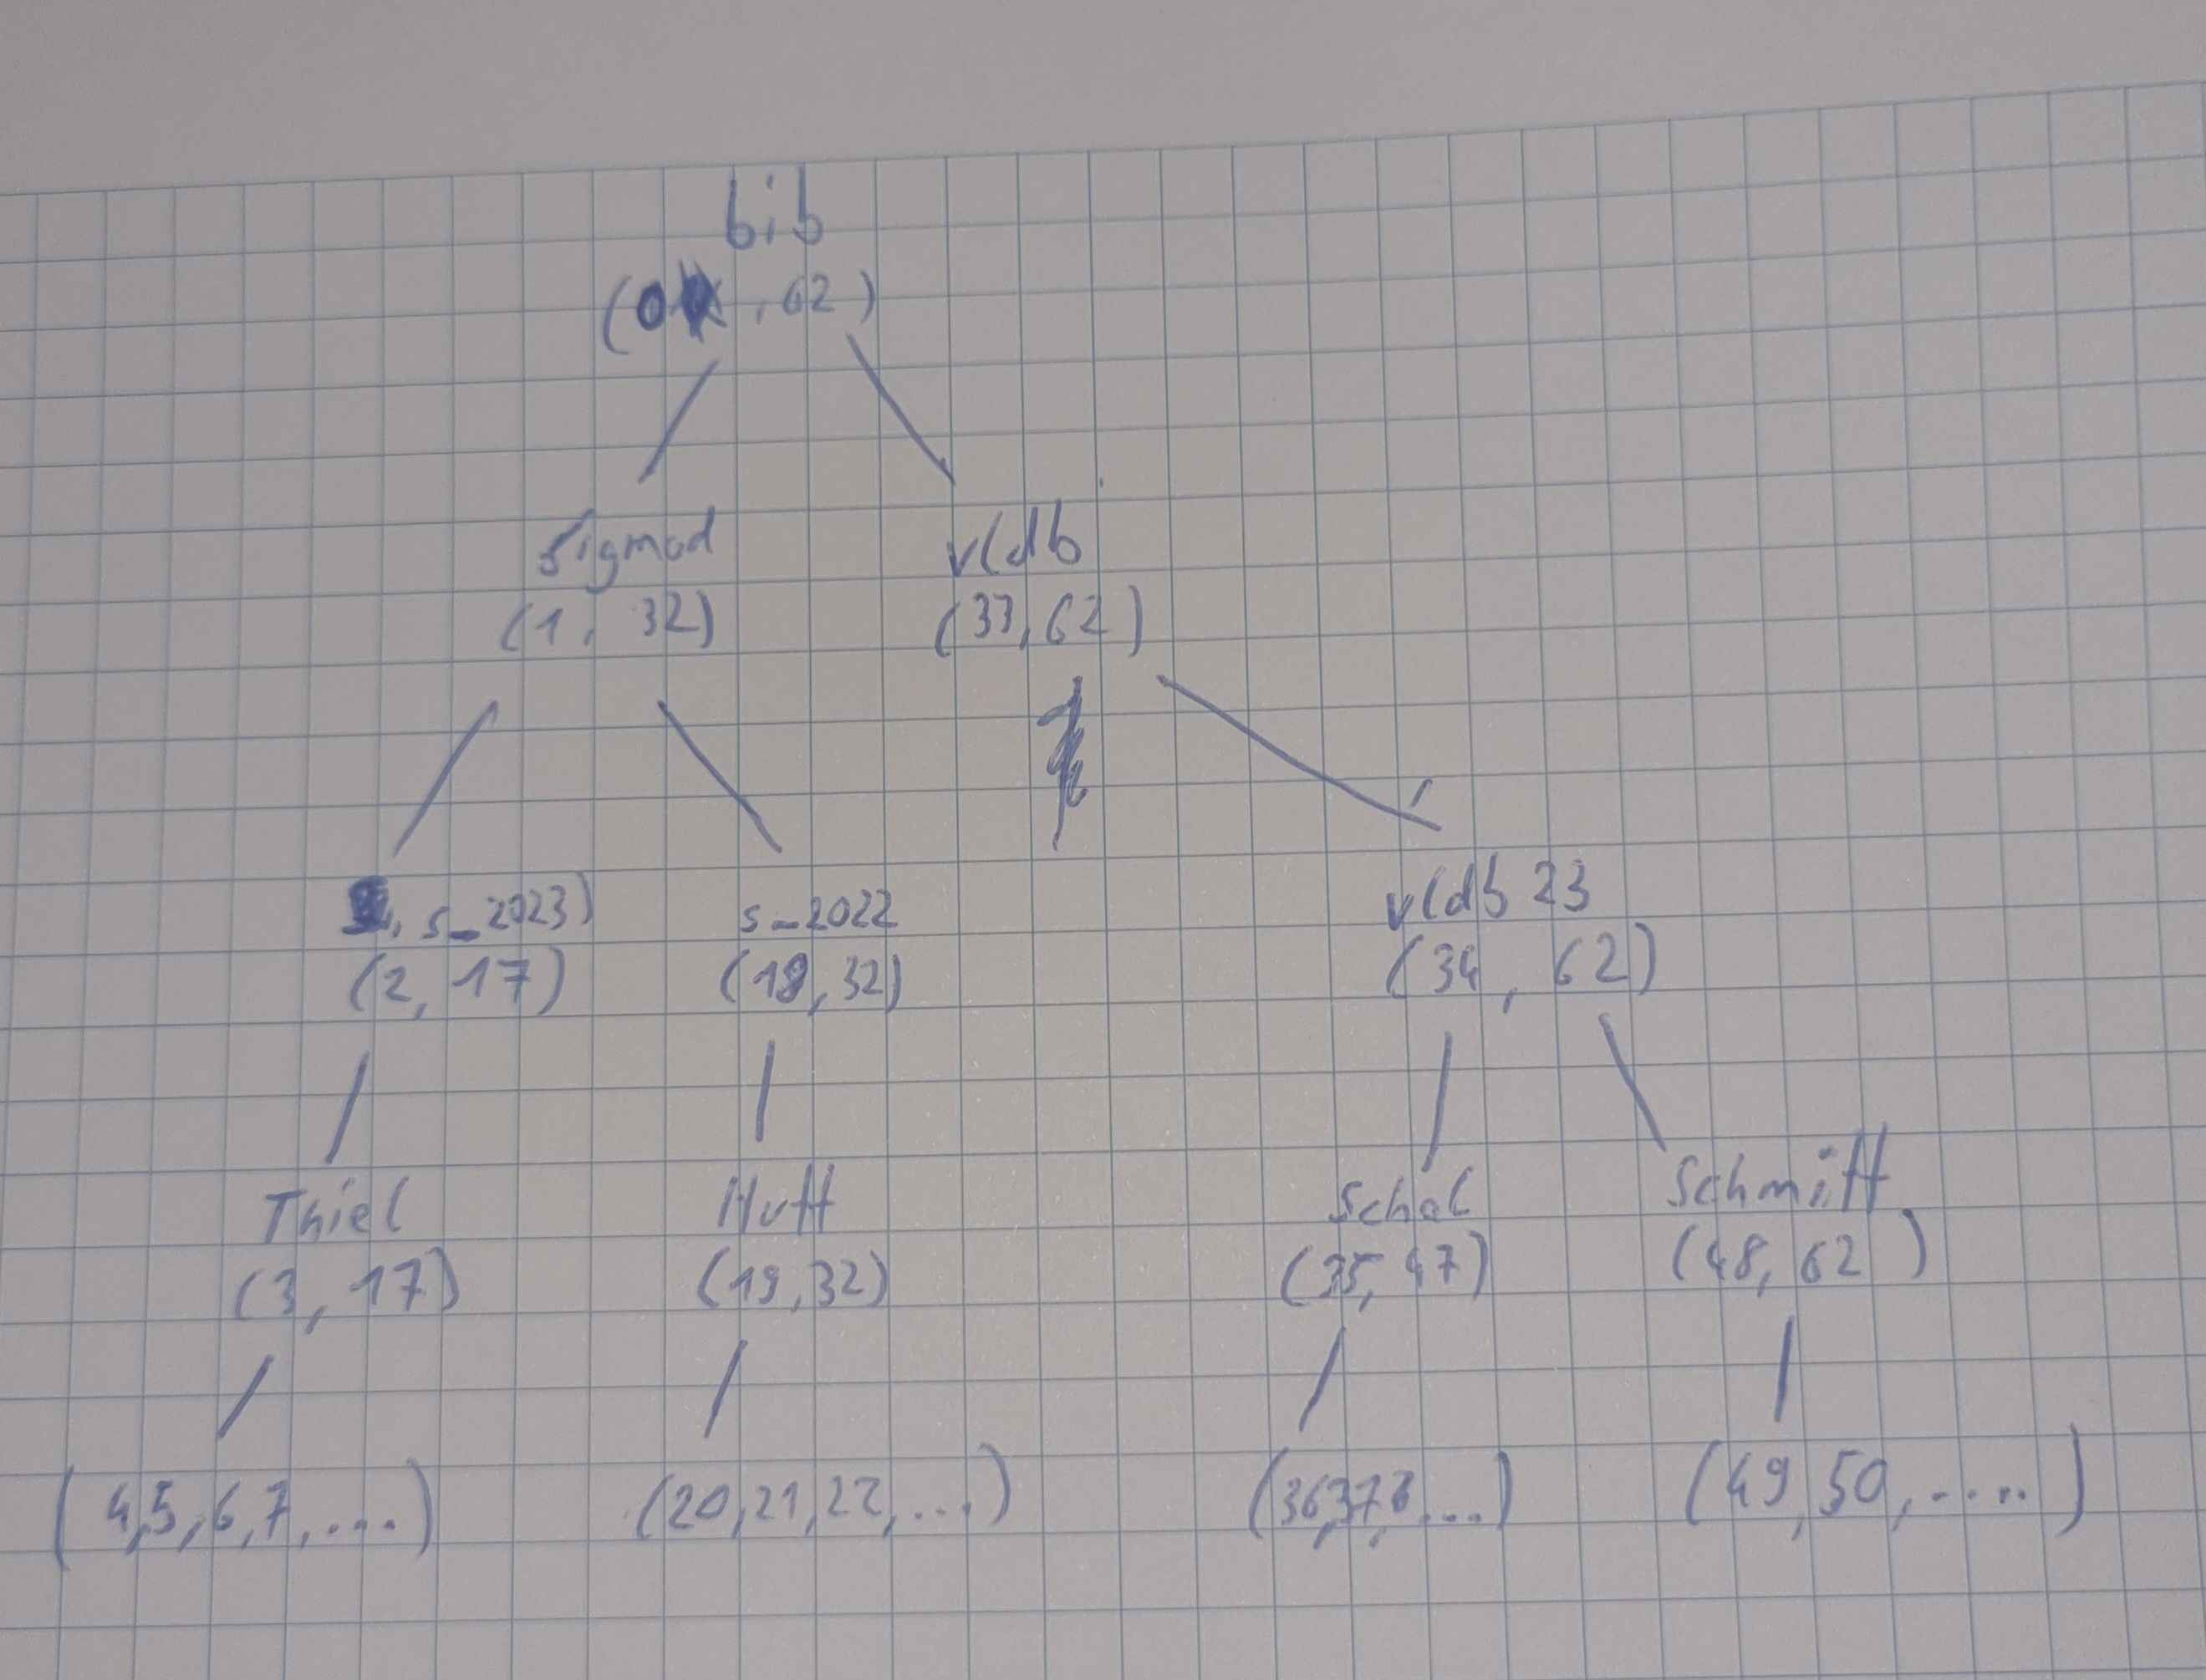
\includegraphics[width=\linewidth]{PrePostBaum.png}
	\caption{Händische Berechnung Pre/Post Baum}\label{fig:node}
\end{figure}

\newpage

\subsection*{Achse als Fenster (2 Punkt)}
Zeigen Sie, dass die Berechnung der Achsen für die Beispiele aus Phase 1 hier die gleichen Ergebnisse erzeugen:

\begin{table}[h]
	\centering
		\begin{center}
			\begin{tabular}{ l | c c }
				\toprule
				Achse & Ergebnisknoten ID's & Ergebnisgröße\\
				\midrule
				ancestor & \{48, 34, 33, 0\} & 4 \\
				descendants & \{35, 36, 37, 38, ..., 62\} & 28 \\
				following SchmittKAMM23 & \emptyset & 0 \\
				preceeding SchmittKAMM23 & \{35\} & 1 \\
				following SchalerHS23 & \{48\} & 1 \\
				preceeding SchalerHS23 & \emptyset & 0 \\
				\bottomrule
			\end{tabular}
			\end{center}
	\caption{Ergebnisse der XPath-Berechnung auf Edge Modell aus Phase 1}
	\label{tab:ErgebnisseDerXPathBerechnug}
\end{table}

\begin{table}[h]
	\centering
		\begin{center}
			\begin{tabular}{ l | c c }
				\toprule
				Achse & Ergebnisknoten ID's & Ergebnisgröße\\
				\midrule
				ancestor & \{48, 34, 33, 0\} & 4 \\
				descendants & \{35, 36, 37, 38, ..., 62\} & 28 \\
				following SchmittKAMM23 & \emptyset & 0 \\
				preceeding SchmittKAMM23 & \{35\} & 1 \\
				following SchalerHS23 & \{48\} & 1 \\
				preceeding SchalerHS23 & \emptyset & 0 \\
				\bottomrule
			\end{tabular}
			\end{center}
	\caption{Ergebnisse der XPath-Berechnung des XPath-Accelerators aus Phase 2}
	\label{tab:ErgebnisseDerXPathBerechnug1}
\end{table}

\subsection*{Zeitmamagement}

Benötigte Zeit pro Person (nur Phase 2):
\textbf{Alexander Weilert: 15h} \\
\textbf{Dragana Jovanovic: 14h}


\end{document}
